% Created by tikzDevice version 0.10.1 on 2016-08-16 17:16:34
% !TEX encoding = UTF-8 Unicode
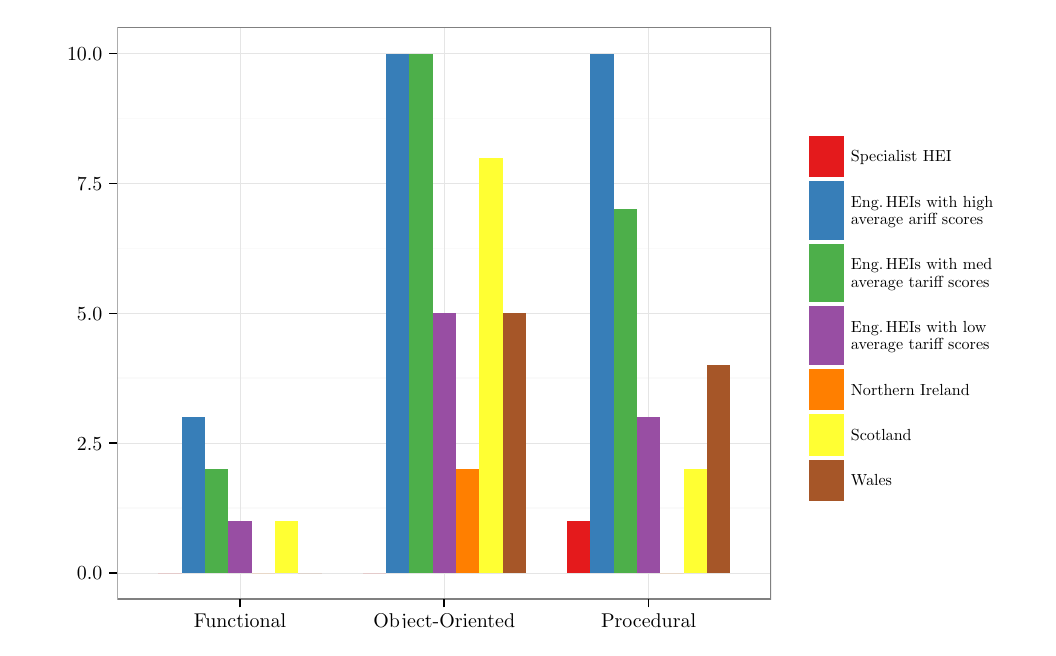
\begin{tikzpicture}[x=1pt,y=1pt]
\definecolor{fillColor}{RGB}{255,255,255}
\path[use as bounding box,fill=fillColor,fill opacity=0.00] (0,0) rectangle (361.35,216.81);
\begin{scope}
\path[clip] (  0.00,  0.00) rectangle (361.35,216.81);
\definecolor{drawColor}{RGB}{255,255,255}
\definecolor{fillColor}{RGB}{255,255,255}

\path[draw=drawColor,line width= 0.6pt,line join=round,line cap=round,fill=fillColor] (  0.00,  0.00) rectangle (361.35,216.81);
\end{scope}
\begin{scope}
\path[clip] ( 32.42, 10.36) rectangle (268.65,216.81);
\definecolor{fillColor}{RGB}{255,255,255}

\path[fill=fillColor] ( 32.42, 10.36) rectangle (268.65,216.81);
\definecolor{drawColor}{gray}{0.98}

\path[draw=drawColor,line width= 0.6pt,line join=round] ( 32.42, 43.20) --
	(268.65, 43.20);

\path[draw=drawColor,line width= 0.6pt,line join=round] ( 32.42, 90.12) --
	(268.65, 90.12);

\path[draw=drawColor,line width= 0.6pt,line join=round] ( 32.42,137.04) --
	(268.65,137.04);

\path[draw=drawColor,line width= 0.6pt,line join=round] ( 32.42,183.97) --
	(268.65,183.97);
\definecolor{drawColor}{gray}{0.90}

\path[draw=drawColor,line width= 0.2pt,line join=round] ( 32.42, 19.74) --
	(268.65, 19.74);

\path[draw=drawColor,line width= 0.2pt,line join=round] ( 32.42, 66.66) --
	(268.65, 66.66);

\path[draw=drawColor,line width= 0.2pt,line join=round] ( 32.42,113.58) --
	(268.65,113.58);

\path[draw=drawColor,line width= 0.2pt,line join=round] ( 32.42,160.51) --
	(268.65,160.51);

\path[draw=drawColor,line width= 0.2pt,line join=round] ( 32.42,207.43) --
	(268.65,207.43);

\path[draw=drawColor,line width= 0.2pt,line join=round] ( 76.72, 10.36) --
	( 76.72,216.81);

\path[draw=drawColor,line width= 0.2pt,line join=round] (150.54, 10.36) --
	(150.54,216.81);

\path[draw=drawColor,line width= 0.2pt,line join=round] (224.36, 10.36) --
	(224.36,216.81);
\definecolor{fillColor}{RGB}{228,26,28}

\path[fill=fillColor] ( 47.19, 19.74) rectangle ( 55.62, 19.74);
\definecolor{fillColor}{RGB}{55,126,184}

\path[fill=fillColor] ( 55.62, 19.74) rectangle ( 64.06, 76.05);
\definecolor{fillColor}{RGB}{77,175,74}

\path[fill=fillColor] ( 64.06, 19.74) rectangle ( 72.50, 57.28);
\definecolor{fillColor}{RGB}{152,78,163}

\path[fill=fillColor] ( 72.50, 19.74) rectangle ( 80.93, 38.51);
\definecolor{fillColor}{RGB}{255,127,0}

\path[fill=fillColor] ( 80.93, 19.74) rectangle ( 89.37, 19.74);
\definecolor{fillColor}{RGB}{255,255,51}

\path[fill=fillColor] ( 89.37, 19.74) rectangle ( 97.81, 38.51);
\definecolor{fillColor}{RGB}{166,86,40}

\path[fill=fillColor] ( 97.81, 19.74) rectangle (106.24, 19.74);
\definecolor{fillColor}{RGB}{228,26,28}

\path[fill=fillColor] (121.01, 19.74) rectangle (129.44, 19.74);
\definecolor{fillColor}{RGB}{55,126,184}

\path[fill=fillColor] (129.44, 19.74) rectangle (137.88,207.43);
\definecolor{fillColor}{RGB}{77,175,74}

\path[fill=fillColor] (137.88, 19.74) rectangle (146.32,207.43);
\definecolor{fillColor}{RGB}{152,78,163}

\path[fill=fillColor] (146.32, 19.74) rectangle (154.75,113.58);
\definecolor{fillColor}{RGB}{255,127,0}

\path[fill=fillColor] (154.75, 19.74) rectangle (163.19, 57.28);
\definecolor{fillColor}{RGB}{255,255,51}

\path[fill=fillColor] (163.19, 19.74) rectangle (171.63,169.89);
\definecolor{fillColor}{RGB}{166,86,40}

\path[fill=fillColor] (171.63, 19.74) rectangle (180.06,113.58);
\definecolor{fillColor}{RGB}{228,26,28}

\path[fill=fillColor] (194.83, 19.74) rectangle (203.27, 38.51);
\definecolor{fillColor}{RGB}{55,126,184}

\path[fill=fillColor] (203.27, 19.74) rectangle (211.70,207.43);
\definecolor{fillColor}{RGB}{77,175,74}

\path[fill=fillColor] (211.70, 19.74) rectangle (220.14,151.12);
\definecolor{fillColor}{RGB}{152,78,163}

\path[fill=fillColor] (220.14, 19.74) rectangle (228.58, 76.05);
\definecolor{fillColor}{RGB}{255,127,0}

\path[fill=fillColor] (228.58, 19.74) rectangle (237.01, 19.74);
\definecolor{fillColor}{RGB}{255,255,51}

\path[fill=fillColor] (237.01, 19.74) rectangle (245.45, 57.28);
\definecolor{fillColor}{RGB}{166,86,40}

\path[fill=fillColor] (245.45, 19.74) rectangle (253.89, 94.82);
\definecolor{drawColor}{gray}{0.50}

\path[draw=drawColor,line width= 0.6pt,line join=round,line cap=round] ( 32.42, 10.36) rectangle (268.65,216.81);
\end{scope}
\begin{scope}
\path[clip] (  0.00,  0.00) rectangle (361.35,216.81);
\definecolor{drawColor}{RGB}{0,0,0}

\node[text=drawColor,anchor=base east,inner sep=0pt, outer sep=0pt, scale=  0.72] at ( 27.02, 17.26) {0.0};

\node[text=drawColor,anchor=base east,inner sep=0pt, outer sep=0pt, scale=  0.72] at ( 27.02, 64.18) {2.5};

\node[text=drawColor,anchor=base east,inner sep=0pt, outer sep=0pt, scale=  0.72] at ( 27.02,111.10) {5.0};

\node[text=drawColor,anchor=base east,inner sep=0pt, outer sep=0pt, scale=  0.72] at ( 27.02,158.03) {7.5};

\node[text=drawColor,anchor=base east,inner sep=0pt, outer sep=0pt, scale=  0.72] at ( 27.02,204.95) {10.0};
\end{scope}
\begin{scope}
\path[clip] (  0.00,  0.00) rectangle (361.35,216.81);
\definecolor{drawColor}{RGB}{0,0,0}

\path[draw=drawColor,line width= 0.6pt,line join=round] ( 29.42, 19.74) --
	( 32.42, 19.74);

\path[draw=drawColor,line width= 0.6pt,line join=round] ( 29.42, 66.66) --
	( 32.42, 66.66);

\path[draw=drawColor,line width= 0.6pt,line join=round] ( 29.42,113.58) --
	( 32.42,113.58);

\path[draw=drawColor,line width= 0.6pt,line join=round] ( 29.42,160.51) --
	( 32.42,160.51);

\path[draw=drawColor,line width= 0.6pt,line join=round] ( 29.42,207.43) --
	( 32.42,207.43);
\end{scope}
\begin{scope}
\path[clip] (  0.00,  0.00) rectangle (361.35,216.81);
\definecolor{drawColor}{RGB}{0,0,0}

\path[draw=drawColor,line width= 0.6pt,line join=round] ( 76.72,  7.36) --
	( 76.72, 10.36);

\path[draw=drawColor,line width= 0.6pt,line join=round] (150.54,  7.36) --
	(150.54, 10.36);

\path[draw=drawColor,line width= 0.6pt,line join=round] (224.36,  7.36) --
	(224.36, 10.36);
\end{scope}
\begin{scope}
\path[clip] (  0.00,  0.00) rectangle (361.35,216.81);
\definecolor{drawColor}{RGB}{0,0,0}

\node[text=drawColor,anchor=base,inner sep=0pt, outer sep=0pt, scale=  0.72] at ( 76.72,  0.00) {Functional};

\node[text=drawColor,anchor=base,inner sep=0pt, outer sep=0pt, scale=  0.72] at (150.54,  0.00) {Object-Oriented};

\node[text=drawColor,anchor=base,inner sep=0pt, outer sep=0pt, scale=  0.72] at (224.36,  0.00) {Procedural};
\end{scope}
\begin{scope}
\path[clip] (  0.00,  0.00) rectangle (361.35,216.81);
\definecolor{fillColor}{RGB}{255,255,255}

\path[fill=fillColor] (277.19, 40.75) rectangle (352.81,186.42);
\end{scope}
\begin{scope}
\path[clip] (  0.00,  0.00) rectangle (361.35,216.81);
\definecolor{fillColor}{RGB}{228,26,28}

\path[fill=fillColor] (282.16,162.84) rectangle (294.97,177.83);
\end{scope}
\begin{scope}
\path[clip] (  0.00,  0.00) rectangle (361.35,216.81);
\definecolor{fillColor}{RGB}{55,126,184}

\path[fill=fillColor] (282.16,140.21) rectangle (294.97,161.42);
\end{scope}
\begin{scope}
\path[clip] (  0.00,  0.00) rectangle (361.35,216.81);
\definecolor{fillColor}{RGB}{77,175,74}

\path[fill=fillColor] (282.16,117.58) rectangle (294.97,138.79);
\end{scope}
\begin{scope}
\path[clip] (  0.00,  0.00) rectangle (361.35,216.81);
\definecolor{fillColor}{RGB}{152,78,163}

\path[fill=fillColor] (282.16, 94.95) rectangle (294.97,116.16);
\end{scope}
\begin{scope}
\path[clip] (  0.00,  0.00) rectangle (361.35,216.81);
\definecolor{fillColor}{RGB}{255,127,0}

\path[fill=fillColor] (282.16, 78.54) rectangle (294.97, 93.53);
\end{scope}
\begin{scope}
\path[clip] (  0.00,  0.00) rectangle (361.35,216.81);
\definecolor{fillColor}{RGB}{255,255,51}

\path[fill=fillColor] (282.16, 62.14) rectangle (294.97, 77.12);
\end{scope}
\begin{scope}
\path[clip] (  0.00,  0.00) rectangle (361.35,216.81);
\definecolor{fillColor}{RGB}{166,86,40}

\path[fill=fillColor] (282.16, 45.73) rectangle (294.97, 60.71);
\end{scope}
\begin{scope}
\path[clip] (  0.00,  0.00) rectangle (361.35,216.81);
\definecolor{drawColor}{RGB}{0,0,0}

\node[text=drawColor,anchor=base west,inner sep=0pt, outer sep=0pt, scale=  0.58] at (297.49,174.57) {};

\node[text=drawColor,anchor=base west,inner sep=0pt, outer sep=0pt, scale=  0.58] at (297.49,168.35) {Specialist HEI};

\node[text=drawColor,anchor=base west,inner sep=0pt, outer sep=0pt, scale=  0.58] at (297.49,162.13) {};
\end{scope}
\begin{scope}
\path[clip] (  0.00,  0.00) rectangle (361.35,216.81);
\definecolor{drawColor}{RGB}{0,0,0}

\node[text=drawColor,anchor=base west,inner sep=0pt, outer sep=0pt, scale=  0.58] at (297.49,158.16) {};

\node[text=drawColor,anchor=base west,inner sep=0pt, outer sep=0pt, scale=  0.58] at (297.49,151.94) {Eng.\,HEIs with high};

\node[text=drawColor,anchor=base west,inner sep=0pt, outer sep=0pt, scale=  0.58] at (297.49,145.72) {average ariff scores};

\node[text=drawColor,anchor=base west,inner sep=0pt, outer sep=0pt, scale=  0.58] at (297.49,139.50) {};
\end{scope}
\begin{scope}
\path[clip] (  0.00,  0.00) rectangle (361.35,216.81);
\definecolor{drawColor}{RGB}{0,0,0}

\node[text=drawColor,anchor=base west,inner sep=0pt, outer sep=0pt, scale=  0.58] at (297.49,135.53) {};

\node[text=drawColor,anchor=base west,inner sep=0pt, outer sep=0pt, scale=  0.58] at (297.49,129.31) {Eng.\,HEIs with med};

\node[text=drawColor,anchor=base west,inner sep=0pt, outer sep=0pt, scale=  0.58] at (297.49,123.09) {average tariff scores};

\node[text=drawColor,anchor=base west,inner sep=0pt, outer sep=0pt, scale=  0.58] at (297.49,116.87) {};
\end{scope}
\begin{scope}
\path[clip] (  0.00,  0.00) rectangle (361.35,216.81);
\definecolor{drawColor}{RGB}{0,0,0}

\node[text=drawColor,anchor=base west,inner sep=0pt, outer sep=0pt, scale=  0.58] at (297.49,112.90) {};

\node[text=drawColor,anchor=base west,inner sep=0pt, outer sep=0pt, scale=  0.58] at (297.49,106.68) {Eng.\,HEIs with low};

\node[text=drawColor,anchor=base west,inner sep=0pt, outer sep=0pt, scale=  0.58] at (297.49,100.46) {average tariff scores};

\node[text=drawColor,anchor=base west,inner sep=0pt, outer sep=0pt, scale=  0.58] at (297.49, 94.24) {};
\end{scope}
\begin{scope}
\path[clip] (  0.00,  0.00) rectangle (361.35,216.81);
\definecolor{drawColor}{RGB}{0,0,0}

\node[text=drawColor,anchor=base west,inner sep=0pt, outer sep=0pt, scale=  0.58] at (297.49, 90.28) {};

\node[text=drawColor,anchor=base west,inner sep=0pt, outer sep=0pt, scale=  0.58] at (297.49, 84.05) {Northern Ireland};

\node[text=drawColor,anchor=base west,inner sep=0pt, outer sep=0pt, scale=  0.58] at (297.49, 77.83) {};
\end{scope}
\begin{scope}
\path[clip] (  0.00,  0.00) rectangle (361.35,216.81);
\definecolor{drawColor}{RGB}{0,0,0}

\node[text=drawColor,anchor=base west,inner sep=0pt, outer sep=0pt, scale=  0.58] at (297.49, 73.87) {};

\node[text=drawColor,anchor=base west,inner sep=0pt, outer sep=0pt, scale=  0.58] at (297.49, 67.65) {Scotland};

\node[text=drawColor,anchor=base west,inner sep=0pt, outer sep=0pt, scale=  0.58] at (297.49, 61.42) {};
\end{scope}
\begin{scope}
\path[clip] (  0.00,  0.00) rectangle (361.35,216.81);
\definecolor{drawColor}{RGB}{0,0,0}

\node[text=drawColor,anchor=base west,inner sep=0pt, outer sep=0pt, scale=  0.58] at (297.49, 57.46) {};

\node[text=drawColor,anchor=base west,inner sep=0pt, outer sep=0pt, scale=  0.58] at (297.49, 51.24) {Wales};

\node[text=drawColor,anchor=base west,inner sep=0pt, outer sep=0pt, scale=  0.58] at (297.49, 45.02) {};
\end{scope}
\end{tikzpicture}
